%% print or electronic
\documentclass[ms,electronic,double]{nuthesis}

%% Needed to typset the math in this sample
\usepackage{amsmath}
\usepackage{amsfonts}
%% Let's use a different font
\usepackage[sc,osf]{mathpazo}

%% Makes things look better
\usepackage{microtype}

%% Makes things look better
\usepackage{booktabs}

%% Gives us extra list environments
\usepackage{paralist}

%% Be able to include graphicsx
\usepackage{graphicx}

%% If you use hyperref, you need to load memhfixc *after* it.
%% See the memoir docs for details.
\usepackage[%
pdfauthor={Kartik Vedalaveni},
pdftitle={Adaptive Co-Scheduler for highly Dynamic Resource},
pdfsubject={Thesis},
pdfkeywords={LaTeX, Thesis, University of Nebraska, Intelligent Co-Scheduler},
linkcolor=dark-blue,
pagecolor=dark-green,
citecolor=dark-blue,
urlcolor=dark-red,
colorlinks=true,
backref,
plainpages=false,% This helps to fix the issue with hyperref with page numbering
pdfpagelabels% This helps to fix the issue with hyperref with page numbering
]{hyperref}

%% Needed by memoir to fix things with hyperref
\usepackage{memhfixc}

%% Needed to display code 
\usepackage{listings}
\usepackage{algorithmic}
\usepackage{algorithm}
\usepackage{subfig}
\usepackage{url}

%% I like darker colors
\usepackage{color}
\definecolor{dark-red}{rgb}{0.6,0,0}
\definecolor{dark-green}{rgb}{0,0.6,0}
\definecolor{dark-blue}{rgb}{0,0,0.6}

\begin{document}
\frontmatter
\title{Adaptive Co-Scheduler for highly Dynamic Resource}
\author{Kartik Vedalaveni}
\adviser{Dr. David Swanson}
\adviserAbstract{Dr. David Swanson}
\major{Computer Science}
\degreemonth{May}
\degreeyear{2013}
\college{Graduate College}
\university{University Of Nebraska}
\city{Lincoln}
\state{Nebraska}
\doctype{Thesis}
\degree{Master Of Science}
\degreeabbreviation{M.S}
\maketitle

\begin{abstract}
Schedulers come with plethora of features and 
options for customization that fulfills myriad goals of  
clusters and data centers . Most state of the art schedulers does not take into account load of resources 
like RAM, I/O or Network for scheduling purpose. Often there is a need to extend these schedulers to solve 
situations arising from these new use cases either by writing a plugin or by Co-Scheduling.One such 
case is when any resources like I/O, RAM or Network is
throttled and the degradation that occurs as a result of it . With increase in number of entities concurrently 
using the resource, there is a 
need to monitor and schedule concurrent and unscrupulous access to any given resource to prevent 
degradation.These issues that we encounter in real life at Holland Computing Center (CITE) are the 
basis and motivation for tackling this problem and develop an adaptive approach for scheduling 
that is aware of multi-resource throttling, load-balancing across multiple sites and degradation 
with a goal to run clusters at high efficiency and share resources fluidly. 
\end{abstract}

\begin{dedication}
Dedicated to 
\end{dedication}

\begin{acknowledgments}
Thanks
\end{acknowledgments}

\tableofcontents
\newpage
\listoffigures
\listoftables


%%   mainmatter is needed after the ToC, (LoF, and LoT) to set the
%%   page numbering correctly for the main body
\mainmatter

\chapter{Introduction}
Grid Computing as defined by wikipedia is the federation of computer resources from multiple locations
to reach a common goal. The resources come in the form of hardware 
and software that allows us to submit jobs, run the jobs and monitor the jobs on the grid. 
Universities usually have multiple clusters across their campus and these are 
owned by different departments but stand united under the banner of university. 
.Campus grids can be thought of as mini grids in which jobs are spanned across multiple clusters
 based on the need of the user and available computing infrastructure 
across multiple clusters within the computing resources across university.

Modern schedulers used in clusters provide innumerable features for policy making, resource management 
and scheduling, the problem of cluster 
performance degradation that occurs when either of the resource is throttled is a problem that hasn't been 
addressed. The problem of performance degradation when many jobs are scheduled on single system 
either based on processor equivalence or based on number of processor slots. Some of 
these schedulers like maui (CITE) are smart enough to take into account contention of other 
resources like RAM but ultimately convert the 2D vector values of CPU and RAM 
into single scalar value which equals to hard-coding the value or presenting these resources
in a ratio which makes us question effectiveness of such scheduling mechanism. 

Here at Holland Computing Center, at University Of Nebraska-Lincoln we're 
tackling this issue of cluster degradation caused by 
over exploitation of one or more resource and I've come up with a solution by adaptively scheduling 
such highly dynamic resource on the grid across multiple sites by adaptively scaling with respect to
degradation that is encountered and degree of turnaround time of the sites which would help increase 
the throughput of the overall Co-Scheduler that also ensures proper loadbalancing.

Existing schedulers depend on the availability of resources and frequent polling 
of it to determine the slots of scheduling. It should be noted that state of the art 
schedulers like maui/torque, slurm, condor take into account only CPU as a 
resource and the resources like RAM, I/O or Network are either ignored or 
converted into a scalar values which isn't an effective way of tackling the multiple resource scheduling 
problem as their true resource load measure is converted to processor equivalent or ignored. 
We take a turnaround time approach to measure degradation, we define a resource 
to be degraded if and when we submit jobs that results in increasing the 
turnaround time by 25\% . It must be 
noted that there isn't explicit measurement of individual resources of RAM, I/O, 
Network and CPU, there are no resource managers keeping track of these resource. 
The Co-Scheduler is driven by the fact that turnaround time increases when 
concurrent jobs accessing these resources reaches a threshold value which in-turn causes 
degradation and this is the basis for our scheduling.

\begin{figure}[htbp!]
\begin{center}
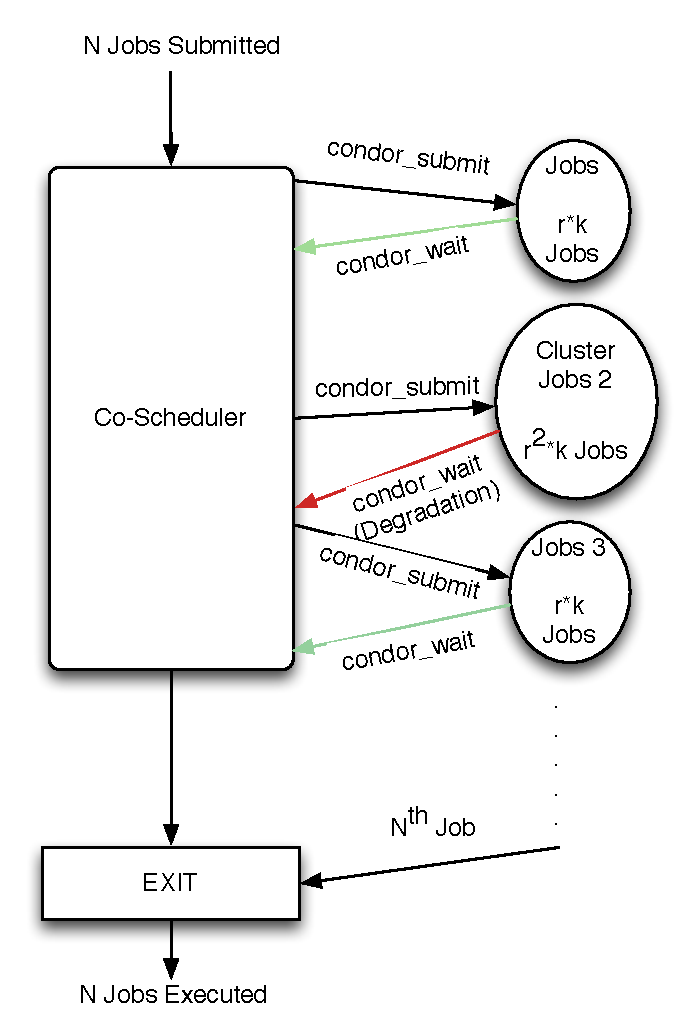
\includegraphics[scale=0.75]{images/degradation_detection}
\caption{Degradation occurrence: Co-Scheduling}
\label{fig:degradationdetect-intro}
\end{center}
\end{figure}

One aspect to Co-Scheduler is degradation detection and management by adapting 
to the throttling of resource another aspect is to efficiently distribute jobs 
across multiple sites which increases the throughput of the Co-Scheduler
. The Co-Scheduler adapts to degradation by backing off submission rates and waiting for random
period of time for the next incremental submission and efficiently 
distributes the jobs and load-balances across multiple sites submitting more 
jobs to a site with lesser turnaround time and also ensuring to submit lesser 
jobs to the sites with larger turnaround time thus efficiently load-balancing 
across multiple sites on a grid.

Finally, Grid environment is a heterogeneous environment, its absolutely necessary
to use API's that are available on all the systems across the grid. To implement such a Co-Scheduler
 we limit ourselves to condor based clusters and utilize libcondorapi. The result is a threaded Co-Scheduler 
that submits to multiple sites concurrently and is aware of multiple-resource degradation and
loadbalances efficiently across multiple sites of the grid. 

Please note that all the references to the Co-Scheduler refers to the adaptive Co-Scheduler designed 
by me.  
\section{Co-Scheduler}

DHTC environment


%% Thesis goes here
\chapter{Background}

\section{High-Throughput Computing} High Throughput Computing, HTC is defined as 
a computing environment that that delivers large amounts of computational
power over a long period of time.  The important factor being over a long period of time which 
differentiates HTC from HPC which focuses on getting large amount of work done in small amount of time.
The workloads that run on condor system doesn't have an objective of  how fast the job can be completed 
but how many times can the job be run in the next few months.In another definition of HTC, European Grid  
Infrastructure defines HTC as a computing paradigm that focuses on the efficient 
execution of large number of loosely coupled tasks.


\section{HTCondor} HTCondor is a distributed system developed by HTCondor team at the 
University of Wisconsin-Madison. It provides High-Throughput Computing environment to sites 
that foster research computing and enables sites to share computing resources when 
computers are idle at a given site. HTCondor system includes a batch queuing 
system,scheduling policy, priority scheme, and resource classifications for a pool of 
computers mainly used for compute-intensive jobs, HTCondor runs on both
 UNIX and windows based workstations that are all connected by a network.  
Although there are other batch schedulers out there for dedicated machines. 
The power of condor comes from  the fact that  the amount of compute power 
represented by sum total of all the 
 non-dedicated desktop workstations sitting on people's desks is sometimes far 
 greater than the compute power of dedicated central resource. There are many 
 unique tools and capabilities in HTCondor which make utilizing resources from 
 non-dedicated systems effective. These capabilities include process checkpoint 
 and migration, remote system calls and ClassAds. HTCondor suit also includes a 
 powerful resource manager with an efficient match-making mechanism that is 
 implemented via ClassAds, which makes HTCondor lucid when compared with other 
 compute schedulers.
 
 
\section{Open Science Grid} Open Science Grid(OSG), provides service and support 
for resource providers and scientific institutions using a distributed fabric of 
high throughout computational services. OSG was created to facilitate data analysis from the 
Large Hadron Collider . OSG doesn't own resources but provides software and services to 
users and enables opportunistic usage and sharing of resources among resource providers.
The main goal of OSG is to advance science through open distributed computing. 
The OSG provides multi-disciplinary partnership to federate local, regional, community and 
national cyber-infrastructures to meet the needs of research and academic communities at all scales.

OSG provides resources and directions to Virtual Organizations(VO's) for the purposes of LHC experiments
and HTC in general. \\

Building a OSG site requires listing background and careful planning. The major 
components of a OSG site includes a Storage Element and Compute Element. \\

Storage elements (SE) manage physical systems, disk caches and hierarchical mass storage 
systems, its an interface for grid jobs to underlying storage Storage Resource Management protocol and Globus 
Grid FTP protocol and others, A storage element requires an underlying storage system like hadoop, xrootd
and a GridFTP server and an SRM interface.\\

A Compute Element(CE) allows grid users to run jobs on your site. It provides a 
bunch of services when run on the gatekeeper. The basic components include 
the GRAM and GridFTP on the same CE host to successfully enable file transfer 
mechanisms of Condor-G.\\


\chapter{Related Work}

\section{Comparison of existing mechanisms}
There might be situations where we can have multiple condor pools and some of 
the pools might be idle . To efficiently utilize the resources condor provides 
some mechanisms like condor flocking and condor job router. These mechanisms 
provide similar functionality to the Co-Scheduler that I designed. In the following sections, we compare 
and evaluate these mechanisms.

\subsection{Condor Flocking}
Flocking refers to a mechanism where jobs that cannot run in its own condor pool 
due to lack of resources runs in another condor pool where resources are 
available. Condor flocking enables load sharing between pools of computers. As 
pointed out by Campus Grids Thesis[CITE 3.1.2]  flocking helps balance large workflows across different pools but not 
necessarily the jobs across these pools because of the scavenging and greedy nature 
of the condor scheduler.

$condor\_schedd$ advertises that it has idle jobs to the remote $condor\_collector$ 
and during the next phase of negotiation, if its found that there are computers 
available then they are allotted to the jobs in the matchmaking phase and the 
jobs then run on the remote pools. It so appears and the local job queue maintains as if 
the jobs are running locally. 

Although Condor flocking has workflow balancing features across multiple condor 
pools it isn't aware of the slower and faster sites/pools. The adaptive Co-Scheduler 
keeps tabs on turnaround time and is aware of which site is faster and which site is slower.If we 
look at the idea that scavenging idle resources increases throughput, it does 
but If we look at the case where jobs are greater than the available slots 
across all the pools, condor flocking stops working here, its role is to only 
scavenge idle computing slots across multiple pools. 

Another aspect where condor flocking might not fare well is when jobs are 
contending for the same resource (CPU, RAM, I/O \& Network). Even though we'll be 
having idle slots on remote pools, condor flocking might not be able to use those 
slots as they'd be degraded because of the contention. In this case again 
Co-Scheduler comes in handy and based on the turnaround time waits for random 
amount of time for degradation to clear and doesn't put heave job load on the 
degraded resource and diverts the jobs elsewhere which in-turn increases the 
throughput.

To conclude, we can say that condor flocking provides features for balancing 
large workflows and doesn't include features that would detect degradation in 
the cluster and also lacks the features that would keep track of information of faster and 
slower sites, which might be exploited to increase the overall throughput of the system. 

\subsection{Condor Job Router}

Condor manual defines the functions of job router to be the following:
\begin{quotation}

The Condor Job Router is an add-on to the $condor\_schedd$ that transforms jobs from one type into 
another according to a configurable policy. 
This process of transforming the jobs is called job routing.
\end{quotation}

Condor Job Router can transform vanilla universe jobs to grid universe jobs and 
as it submits to multiple sites, the rate at which it starts submitting equals 
rate at which the sites execute them thus providing platform to balance large 
workflows across multiple grid sites. Job router sends more jobs to a site if 
the jobs submitted are not idle and stops submitting jobs if the submitted jobs 
sit idle on the remote cluster and Job router is not aware about which site is 
faster of slower.


\begin{figure}[htbp!]
\begin{center}
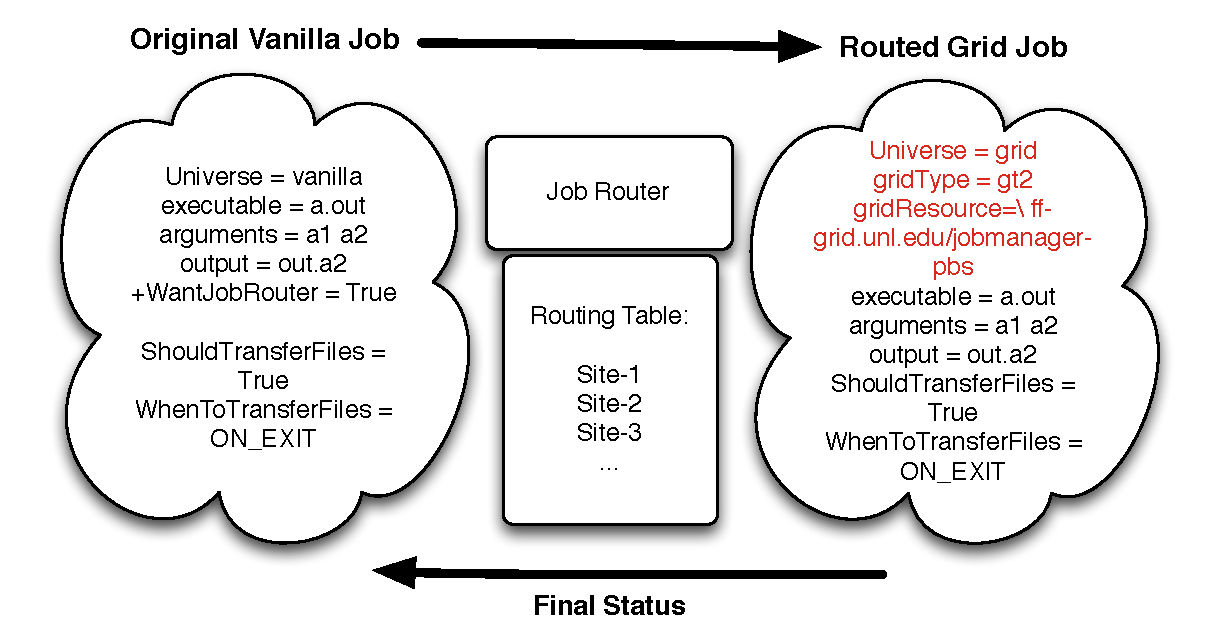
\includegraphics[scale=0.75]{images/jobRouter}
\caption{JobRouter: Transformation of Jobs}
\label{fig:JobRouter}
\end{center}
\end{figure}

A job is transformed to the grid universe by making a copy of the original job 
ClassAd, modifying some attributes of the job , this copy is called the routed 
copy and this routed copy shows up in the job queue with a new job id.

Condor job router utilizes routing table which contains the listings of sites 
the job must be submitted to and the name of the grid resource declared and 
processed during condor config file which is defined by the new ClassAds.

\begin{lstlisting}
  # Now we define each of the routes to send jobs on
JOB_ROUTER_ENTRIES = \
   [ GridResource = "gt5 ff-grid.unl.edu/jobmanager-pbs"; \
     name = "Firefly"; \
   ] \
   [ GridResource = "gt5 tusker-gw1.unl.edu/jobmanager-pbs"; \
     name = "Tusker"; \
   ] \
   [ GridResource = "gt5 pf-grid.unl.edu/jobmanager-condor"; \
     name = "Prairiefire"; \
   ]\

\end{lstlisting}


Condor Job Router seems to be a step up from the Condor Flocking in terms of 
scavenging resources and sending the extra jobs to another condor pool. Condor 
Job Router also maintains the rate of the jobs on remote clusters

\subsection{Co-Scheduler Solution}

%%A table of comparison among all three kinds of mechanisms



\section{Turnaround based scheduling, IIT Roorkee}

\chapter{Design and Implementation of Co-Scheduler}
\section{Capacity based Co-Scheduling}
\section{multi-site turnaround time Co-Scheduling}
\section{Programming APIs}
\subsection{Condor Log Reader and User API}
\subsection{Synchronization Co-Scheduler Code}

\chapter{Evaluation}

\chapter{Conclusion}


%% backmatter is needed at the end of the main body of your thesis to
%% set up page numbering correctly for the remainder of the thesis
\backmatter

%% Start the correct formatting for the appendices
\appendix

%% Appendices go here (if you have them)

%% Bibliography goes here (You better have one)
%% BibTeX is your friend
%% Index go here (if you have one)
%% Bibliography goes here (You better have one)
%% BibTeX is your friend
\bibliographystyle{plain}
\bibliography{KartikThesis}
%% Pull in all the entries in the bibtex file. Is is a useful trick to
%% check all your references.
\nocite{*}

%% Index go here (if you have one)

\end{document}